\documentclass[]{cv-style} % Add 'print' in [] to get print-view
\usepackage{graphicx}
\begin{document}
\header{Y. Müh. Nazım}{Yıldız}
\begin{aside}
\section{.}
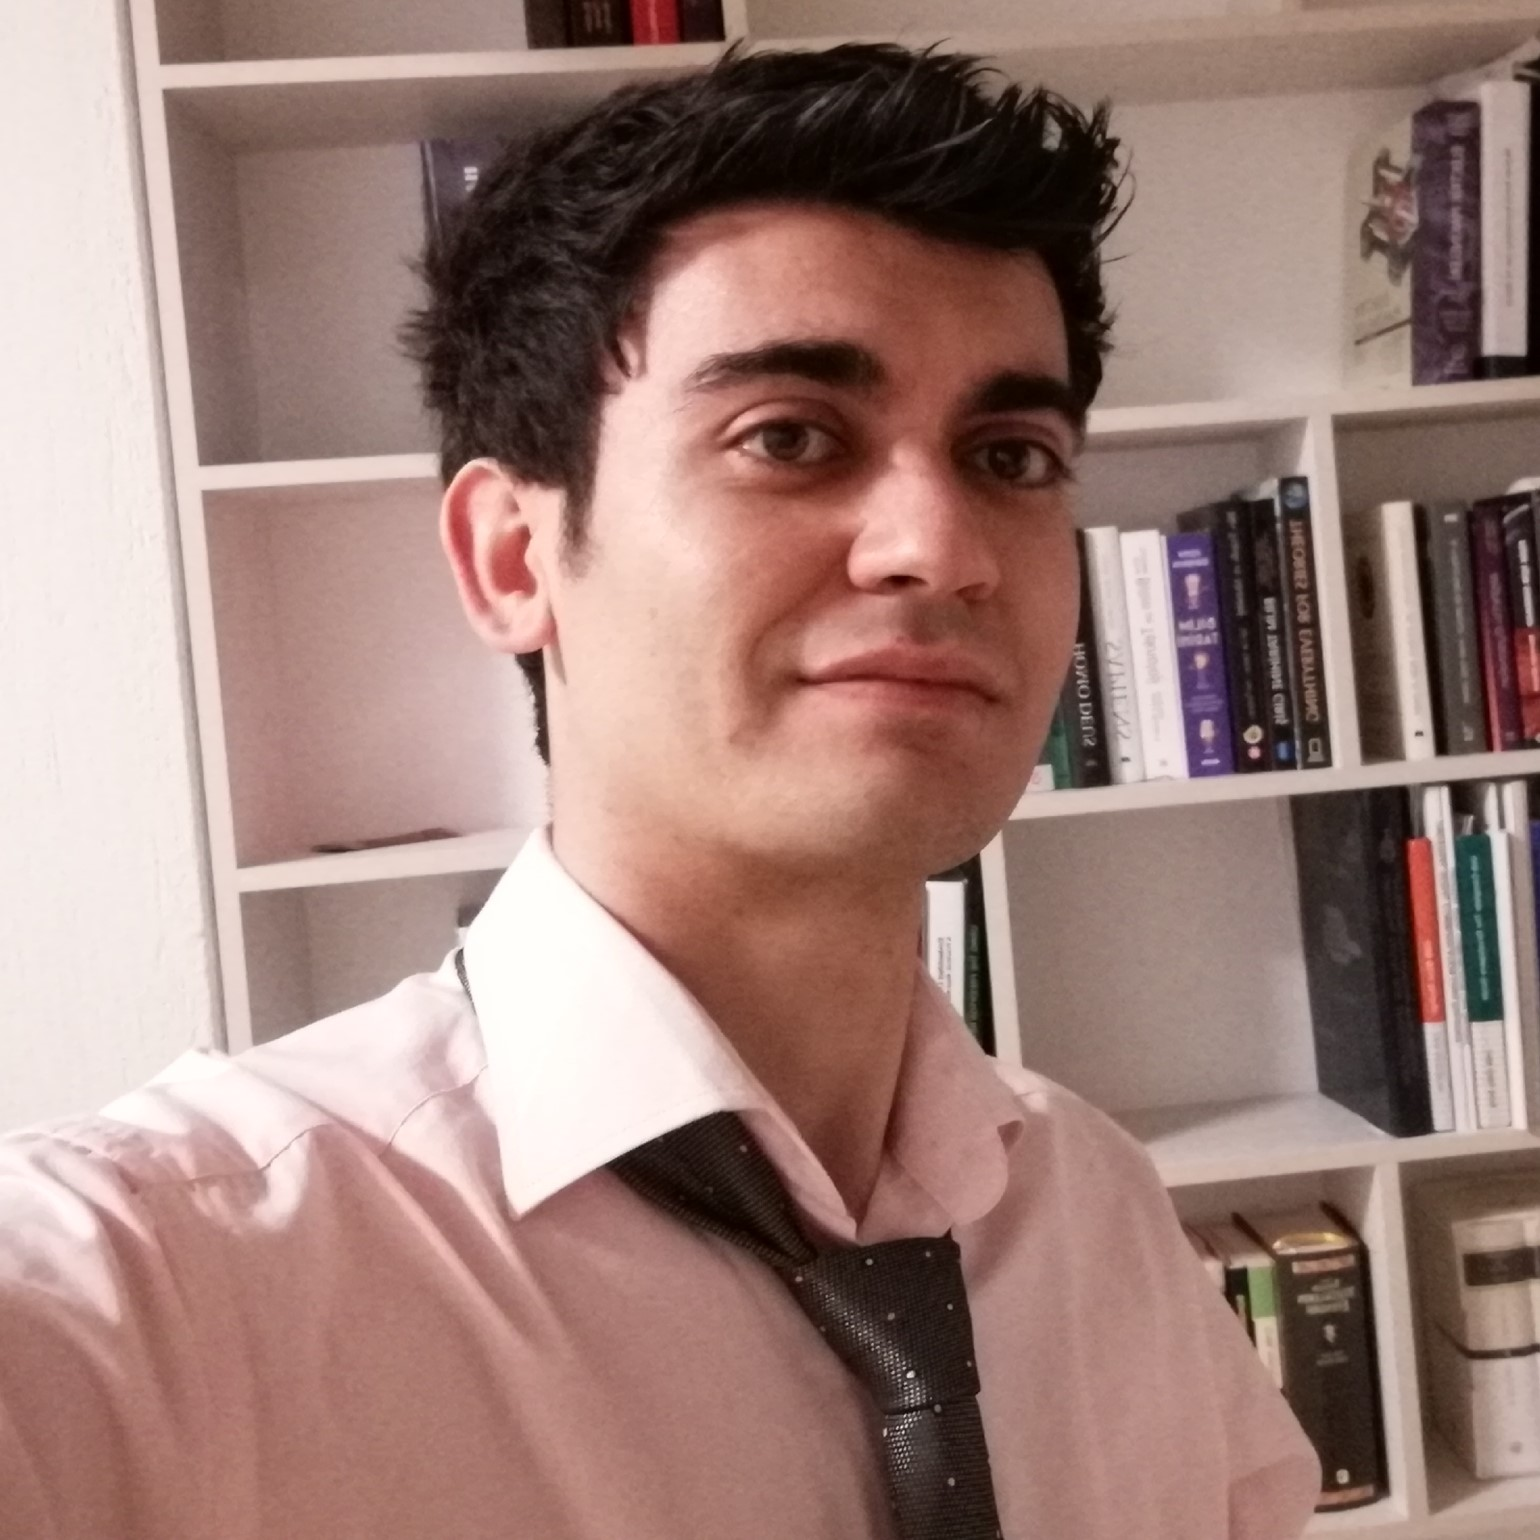
\includegraphics[width=4cm]{photo.jpg}
\section{İletişim}
Atatürk Mah.
952sok. No:32
Bornova/İzmir
~
+90 555 681 8042
+90 232 351 3345
~
nazimyildiz90@gmail.com
\section{Kişisel Bilgiler}
Doğum Yeri: Bulgaristan/Mestanlı
\hspace{0.2mm}
Doğum Tarihi: 30/06/1990
\section{İçeriklerim}
\href{www.nazimyildiz.com}{www.nazimyildiz.com}
\href{https://github.com/namcho}{Github}
\href{https://www.linkedin.com/in/naz%C4%B1m-y%C4%B1ld%C4%B1z-a67b0344/}{Linkedin}
\section{Önemli Özelliklerim}
ASM - ARM
C/C++
Linux Sever
Güç Elektroniği
PCB Tasarımı
Altium Designer
Analog Devre Tasarımı
Matlab
Ansys - Electronics
Latex
Deep-Learning
\end{aside}
\section{Kariyer Hedefim}
  \vspace{-0.2cm}
Bir ya da birkaç üst ligde tasarım yapma arzusu içerisinde, yelkenleri yeteri kadar teorik bilgi ve tecrübe ile dolu, yeni bir limana doğru hareket etmeyi heyecanla bekleyen genç ve deneyimli bir mühendisim. Özellikle derin-öğrenme konularında edinmiş olduğum teorik bilgi ve becerilerimi endüstriyel/askeri/medikal cihazlara entegre edebilme fırsatının verileceği projelerde yer almayı heyecanla beklemekteyim.
\section{Deneyim}
\begin{entrylist}
\entry
  {2013 - Halen}
  {Enko Elektronik A.Ş.}
  {İzmir, Türkiye}
  {\jobtitle{Tasarım Mühendisi}\\
- Kompresör kontrol ürünleri için alt yapı tasarımını tamamladım, istenilen ürün özelliklerine göre ürün ağacını genişletmeyi oldukça kolay hale getirdim
\\- İki adet kompresör ürününün tasarımını tamamladım, üçüncüsünü üzerindeki çalışmalarım devam etmektedir. Kompresörlerin paralel çalışmalarına imkan sağlayan ve eşit yaşlandırma kabiliyeti olan "çoklu-çalıştırma" özelliğini kompresör ürünlerine kazandıran yazılımı geliştirdim. Kompresörlerin kendi aralarındaki bilgi paylaşımı için CANopen haberleşme protokolü tercih edilmiştir
\\- Askeri bir projede kullanılan müşteriye özel Canrouter olarak adlandırılan ürünün hem donanım hem yazılımını geliştirdim. CANBus cihaz adresleri aynı olan birden fazla ECU'nun aynı can-bus haberleşme hattına bağlanıp kontrol edilmesine olanak sağlayan CAN-J1939 standartına uygun bir üründür
\\- Vektör kontrol(FOC) tekniği ile ACIM ve PMAC motorlar için TEYDEB projesi kapsamında farklı mikrodenetleyicilere kolayca taşınabilir yazılım kütüphanesini geliştirdim. Geliştirdiğim bu yazılımın testlerini 4.5kW'lık Femsan firmasının PMAC motorunu kullanarak başarılı bir şekilde tamamladım(2014)
\\- DC/AC micro-İnvertör 1kW gücünde, $\%$98.4 verim, 98.53x86.77mm boyutlarında PCB, 100kHz anahtarlama frekansı, yüksek dv/dt(yükselme eğimi yaklaşık 410V/20ns) özelliklerine sahip hobi çalışmamı tamamladım(07/2021). Detaylar için bknz. Linkedin sayfam - "Öne çıkarılan/Featured" bölümü.}
\end{entrylist}
\section{Eğitim}
\begin{entrylist}
\entry
{2015 - 2018}
{Yüksek Lisans {\normalfont Elektrik ve Elektronik Mühendisliği [3.78 / 4]}}
{Denizli, Türkiye}
{Pamukkale Üniversitesi}
\entry
{2009 - 2013}
{Lisans. {\normalfont Elektrik ve Elektronik Mühendisliği [77.17 / 100]}}
{Denizli, Türkiye}
{Pamukkale Üniversitesi}
\end{entrylist} 
\section{Derin Öğrenme Sertifikalarım}
\begin{entrylist}
    
    \entry
    {2020 Kasım}
    {Deep Learning Specialization}
    {\href{https://www.coursera.org/account/accomplishments/specialization/certificate/R2Y6SR7KCMDX}{R2Y6SR7KCMDX}}
    {Stanford Üniversitesi - Adjunct Professor Andrew Ng [Coursera]}
    
    \entry
    {2020 Kasım}
    {Convolutional Neural Networks}
    {\href{https://www.coursera.org/account/accomplishments/certificate/RUA85RRGYH83}{RUA85RRGYH83}}
    {Stanford Üniversitesi - Adjunct Professor Andrew Ng [Coursera]}
    
    \entry
    {2020 Ekim}
    {Sequence Models}
    {\href{https://www.coursera.org/account/accomplishments/certificate/LXKNTN8MSWFA}{LXKNTN8MSWFA}}
    {Stanford Üniversitesi - Adjunct Professor Andrew Ng [Coursera]}
    
    \entry
    {2020 Nisan}
    {Structuring Machine Learning Projects}
    {\href{https://www.coursera.org/account/accomplishments/certificate/LGQXFPS7MKXW}{LGQXFPS7MKXW}}
    {Stanford Üniversitesi - Adjunct Professor Andrew Ng [Coursera]}
    
    \entry
    {2020 Nisan}
    {Improving Deep Neural Networks}
    {\href{https://www.coursera.org/account/accomplishments/certificate/VERZ2NT3C3HE}{VERZ2NT3C3HE}}
    {Stanford Üniversitesi - Adjunct Professor Andrew Ng [Coursera]}
    
    \entry
    {2020 Mart}
    {Neural Networks and Deep Learning}
    {\href{https://www.coursera.org/account/accomplishments/verify/9QZR6R88ZHPE}{9QZR6R88ZHPE}}
    {Stanford Üniversitesi - Adjunct Professor Andrew Ng [Coursera]}
    
\end{entrylist}
\end{document}